\section{Introduction}
\subsection{Me}
\begin{frame}{Introduction - Me}
\begin{columns}
\column{0.6\textwidth}
Who am I?
\begin{itemize}
\item \insertauthor
\item Integrated Masters in Chemistry at the University of Nottingham
\item Masters with Prof. Nicholas Besley
\item PhD Student at the University of Nottingham
\item Supervisors are 
	\begin{itemize}
		\item Prof. Chris Hayes,
		\item Prof. Jonathan Hirst,
		\item Dr. Christof Jager
		\item Dr. David Rogers
	\end{itemize}
\end{itemize}
\column{0.4\textwidth}
\begin{figure}
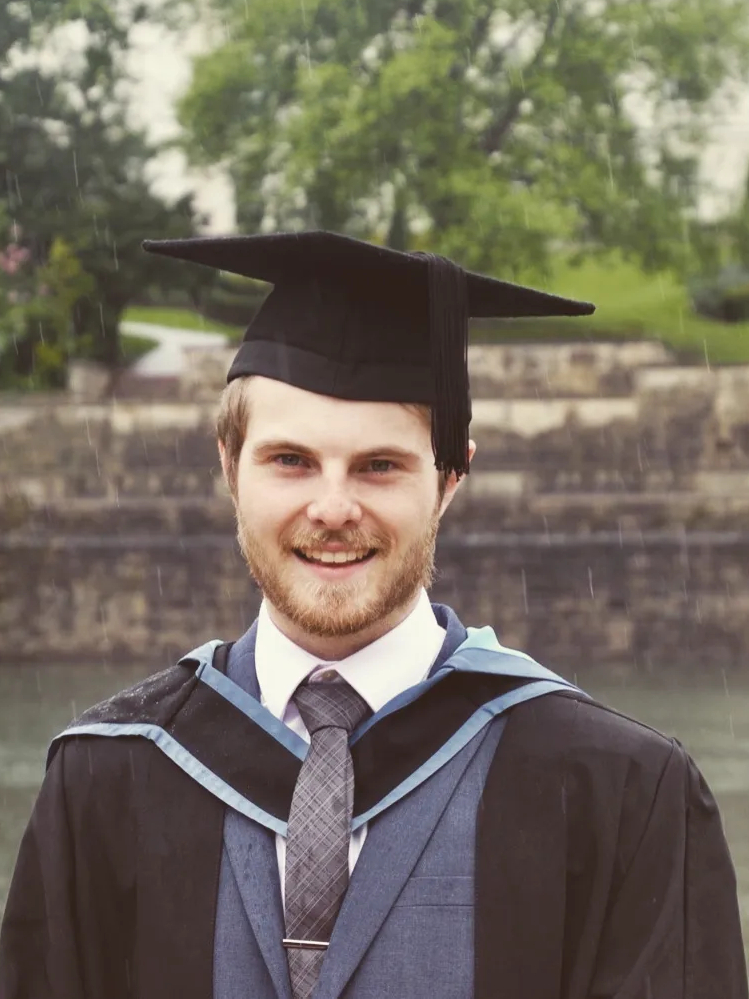
\includegraphics[height=0.8\textheight]{figures/Me/Graduation_Headshot.jpg}
\end{figure}

\end{columns}
\end{frame}

\begin{frame}{Introduction - My Science - Past}
Masters Project:
\begin{columns}
\column{0.5\textwidth}
\begin{figure}
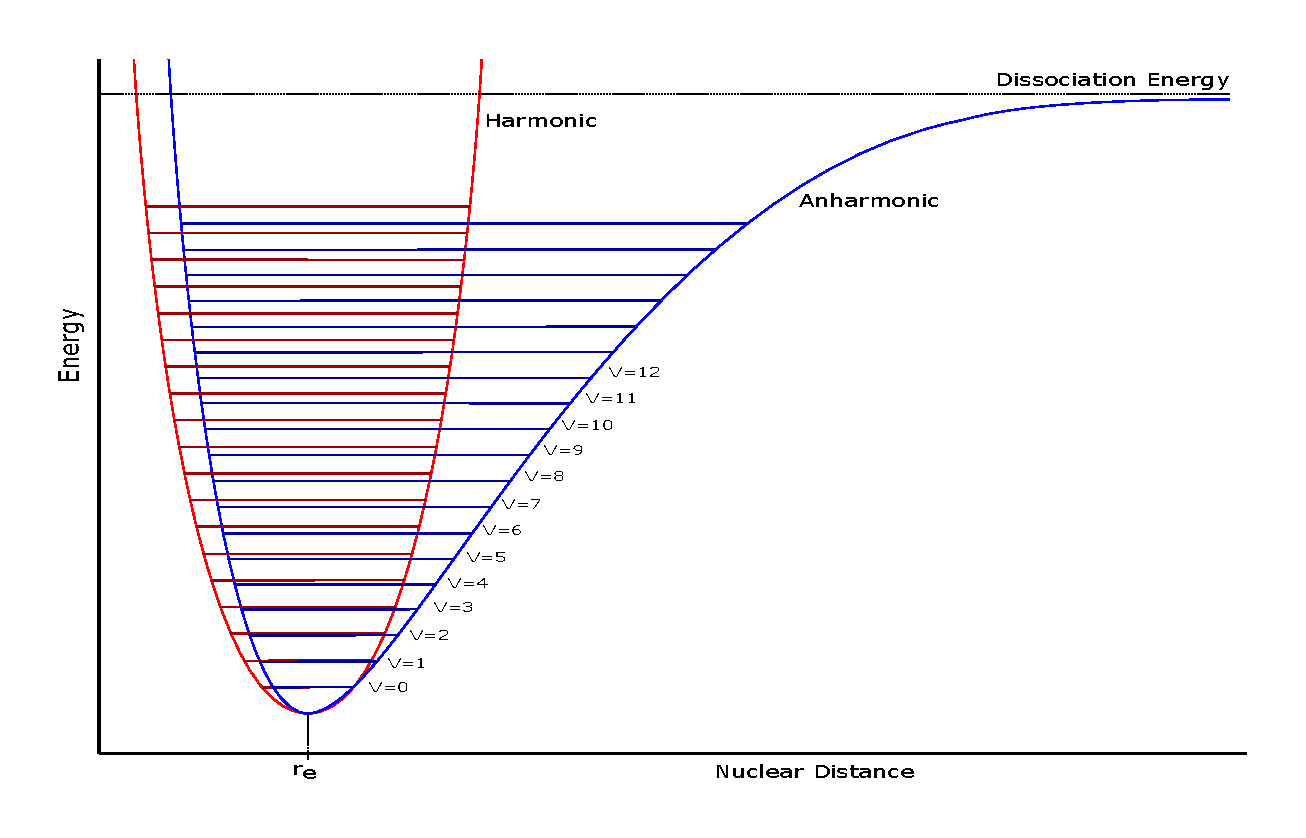
\includegraphics[width=0.7\textwidth]{figures/Me/harmonicoscilator}
\end{figure}
\begin{itemize}
	\item Calculate an anharmonic correction for Raman Spectroscopy
	\item Implement 2\textsuperscript{nd} order numerical derivatives in Fortran90
\end{itemize}

\column{0.5\textwidth}
\begin{figure}
\includegraphics[width=0.7\textwidth]{figures/Me/OptimisedC180.png}
\end{figure}
\begin{itemize}
	\item Calculate Raman Spectrum for Carbon Fullerenes using DFT methods
	\item Compare empirical code to DFT methodology
\end{itemize}

\end{columns}
\end{frame}

\begin{frame}{Introduction - My Science - Current}
\begin{columns}
\column{0.75\textwidth}
\begin{figure}
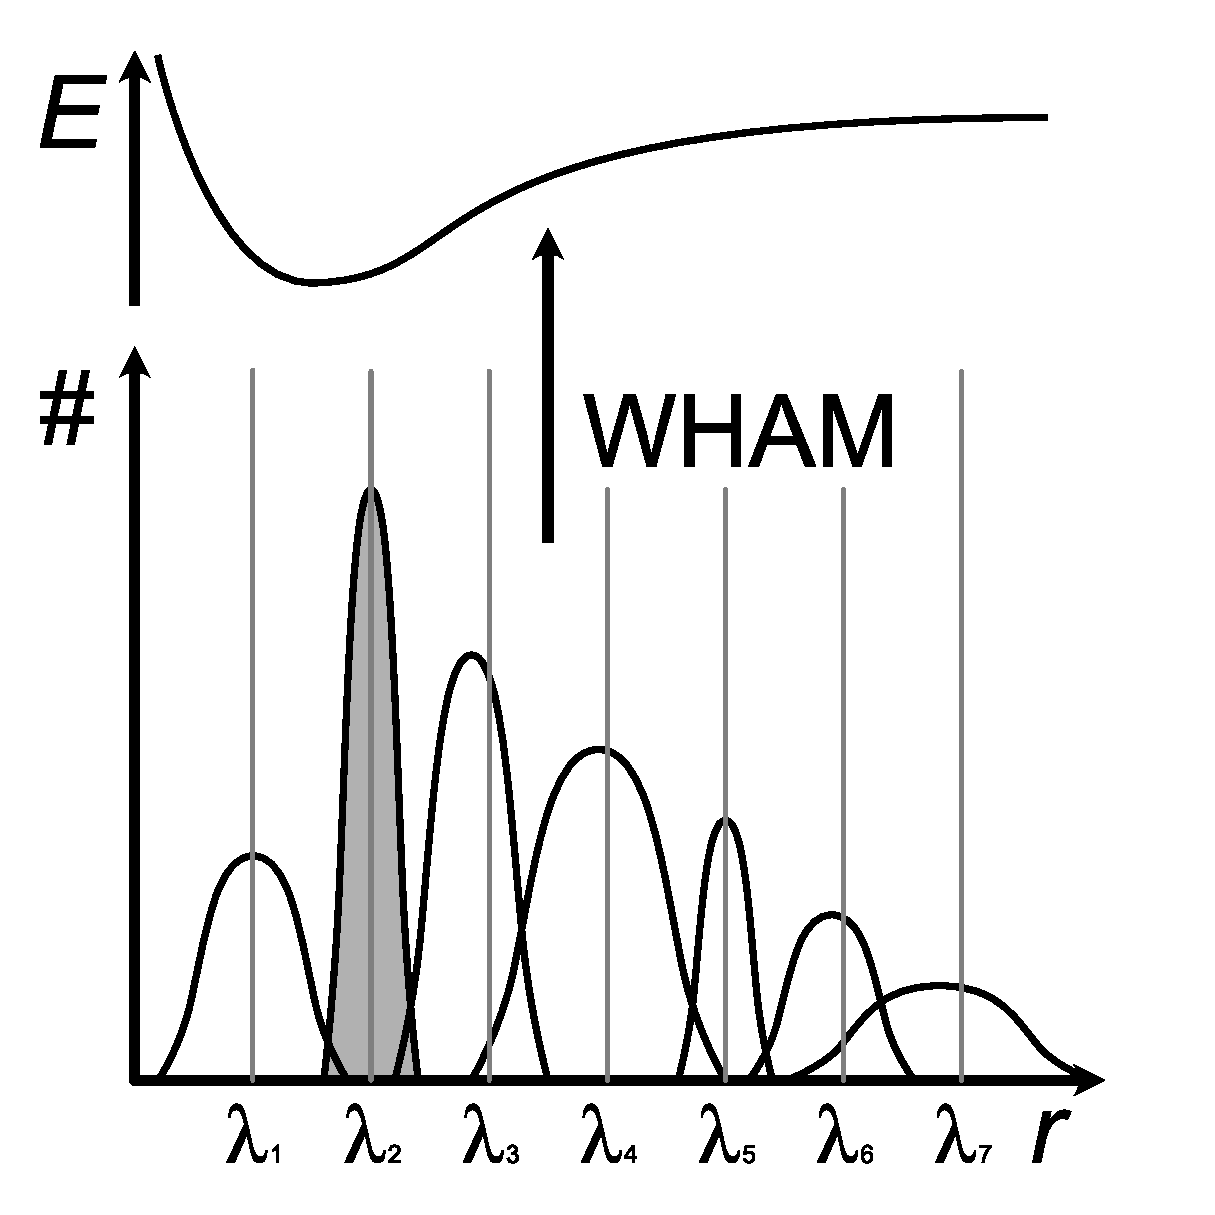
\includegraphics[width=0.4\textwidth]{figures/Me/Wham_Hist}
\end{figure}
\begin{itemize}
	\item Molecular dynamics simulations of Terpene Synthases
	\item Higher level QM/MM Umbrella sampling to obtain Potential Energy Surfaces
\end{itemize}

\column{0.25\textwidth}
\begin{figure}
\includegraphics[width=\textwidth]{figures/Me/FullProtein_coloredLoop.png}
\end{figure}
\end{columns}
\end{frame}

\begin{frame}{Introduction - Molecular Dynamics}
\begin{itemize}
\item \textbf{Self-taught} in Molecular Dynamics

\item Experience of the entire workflow:
	\begin{itemize}
		\item Homology Modelling with AlphaFold and YASARA
		\item Docking using AD4 and Gnina
		\item Simulations using AMBER
		\item QM/MM Simulations with AMBER and QChem
		\item Analysis using GBSA, Umbrella Sampling, clustering etc.
	\end{itemize}
\end{itemize}
\end{frame}
